%\documentclass[fontset=windows]{article}
\documentclass{article}
\usepackage{ctex}
\usepackage{caption}

\title{LSM-KV 项目报告}
\author{卢天宇 519370910127}
\date{2022年 5月 18日}

\usepackage{natbib}
\usepackage{graphicx}
\usepackage{enumitem}
%\bibliographystyle{plain}

\begin{document}

\maketitle

\section{背景介绍}

LSM Tree (Log-structured Merge Tree) 是一种可以高性能执行大量写操作的数据结构。它于 1996 年,在 Patrick O'Neil 等人的一篇论文中被提出。现在,这种数据结构已经广泛应用于数据存储中。Google 的 LevelDB 和Facebook 的 RocksDB 都以 LSM Tree 为核心数据结构。

%这部分应该写LSM-KV这个Project的背景知识和你对这个Project的一些初步理解。 下面是教你如何在 \LaTeX 中插入一张图片。
%这是一个对图片的引用, 图~\ref{fig:universe},以及参考文献~\cite{adams1995hitchhiker}。


%\begin{figure}[h!]
%\centering
%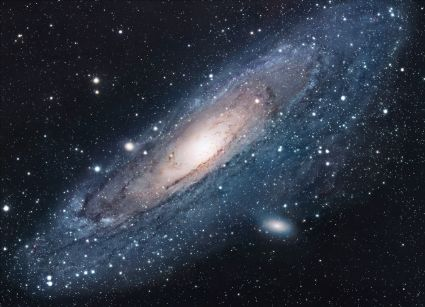
\includegraphics[scale=1.7]{universe}
%\caption{The Universe}
%\label{fig:universe}
%\end{figure}

\section{数据结构和算法概括}


在实现本项目的过程中,我们大量使用了C++标准模板类STL中的数据结构,例如std::vector,std::list,std::pair等等。根据他们的特性,我们在不同的情境下使用二者。例如,对于SSTable的头部缓存,我们利用
\begin{center}
	std::vector$\langle$std::list$\langle$Buffer$\rangle$$\rangle$
\end{center}
的数据结构来进行存储。这是因为,缓存的层级一般只增不减,而且只会在末端插入或删除一层,所以为了达到最大的随机访问效率,我们在最外层使用vector。而对于每一层中的若干SSTable的缓存Buffer,我们使用list进行存储,这是因为我们默认把一层中的Buffer按照时间戳排序,然后,在新写入Buffer的时候,是在末尾写入的,而删除本层溢出的Buffer时,则需要在头部删除,这种同时需要对两端进行操作的情况,使用以链表为实现基础的list更合适。



\section{测试}
%此部分主要是展现你实现的项目的测试,主要分为下面几个子部分。测试部分应当是文字加上测试数据的图片展示。

\subsection{性能测试}\label{test}
在本节中,对LSM-KV系统进行性能测试,分为两个实验,一个测试顺序操作,一个模拟实际情况的随机操作。

对于第一个实验,具体测试方法如下。

首先,初始化系统,内外存中的数据以及缓存数据均为空。然后顺序执行如下三个操作:
\begin{enumerate}
	\item 顺序插入n个键值对,索引值从0至n-1递增,第i个索引的数据为长度为i+1的字符串。
	\item 顺序查找n个索引值,索引值从0至n-1递增。
	\item 顺序删除n个键值对,索引值从0至n-1递增。
\end{enumerate}
进行三组平行实验,每组实验的n值分别设置为5,120、10,240、20,480。

对于第二个实验,具体测试方法如下。
\begin{enumerate}
	\item 在min\_key和max\_key中随机插入n个键值对,数据的长度在min\_length与max\_length之间随机取值。
	\item 在min\_key和max\_key中随机搜索n个索引值。
	\item 在min\_key和max\_key中随机删除n个键值对。
\end{enumerate}
进行三组平行实验,每组实验的n值分别设置为5,120、10,240/20,480。min\_key均设置为,0,max\_key设置为n的2倍。min\_length均设置为1,max\_length设置为n的2倍。

\subsubsection{预期结果}

%在给定下面几个测试的具体数据之前,你应当首先在本节在理论上分析这些测量的结果,此步无需定量,是定性分析,如果此处的分析与后面的具体数据测试有出入,请你给出你理解的导致这种出入的可能性。

\textbf{实验一}

对于存储空间,一方面,在进行插入操作的时候,实际插入的数据量是$O(n^2)$的,所以被分成的sst文件也是$O(n^2)$的。
另一方面,当sst存储的最深层数是k时,由于每层能容纳的sst文件是线性于当前层序数的,于是总共能容纳的sst文件数量是$O(k^2)$的。
于是,最深层数是$O(n)$的。

对于执行时间。
\begin{enumerate}
	\item 顺序插入数据。按上述实验设计进行合并操作时,并不会有索引值交错,或多相同索引值合并的可能。当第0层写入第3个文件时,会触发合并操作,将3个文件一起写入第一层。若第一层原本是满的,则同时也需要将时间戳较小的3个文件删除并写入下层。以此类推,对于每一个已经达到文件数量上限的层级,都需要进行3次写入和删除操作。而触发的总合并次数是正比于sst文件数量的,于是总合并次数是$O(n^2)$的,一次合并的文件读写次数是$O(\textrm{最深层数})=O(n)$的,所以总读写次数是$O(n^3)$的,于是相应的总时间也应与n的值呈现3次方的增长规律。
	\item 顺序查询数据。在第一步的基础上,索引值越小的数据,存储在外存中的层级越深,需要的时间也越多。由于我们的查询保证都能查到有效的索引值,所以每次查询都会有外存读取。具体而言,单次查询的时间复杂度,与所处的层级深度是$O(n)$的,而查询次数是$O(n)$的,故总查询时间应该是$O(n^2)$的。
	\item 顺序删除数据。LSM的删除功能是在GET和PUT已经实现的基础上实现的。先使用GET尝试查找欲删除的索引是否存在,如果存在,则插入\textasciitilde DELETED\textasciitilde 标记。在本实验设计中,GET操作总是会返回成功,于是PUT操作总会得到执行。但是,插入的新数据在合并至最后一层时都会被抹除,于是数据总层数基本不会继续增长。另一方面,删除操作插入的字符串是固定长度的,长度很短,需要累积很多次删除操作才会触发一次写外存,而触发合并操作则更少。综上,总操作时间,应为$O(n^2)$。
\end{enumerate}

\textbf{实验二}

与实验一相仿,仅仅将数据的产生变成了随机的方式。产生重复索引值的概率较小,而大多数情况下,产生的索引值和数据长度都是不同的。则应具有与实验一相似的时间复杂度。

在不同的的n值下,我们用n的值除以平均时延,可以得到单位时间内,系统能够进行的某种操作的数量,我们将测试结果作为对数据结构吞吐量的估计值。


\subsubsection{常规分析}

\begin{enumerate}
    \item %包括Get、Put、Delete操作的延迟,你需要测出不同数据大小时的操作延迟,为了测试的合理性,你应当对每个数据大小测量然后计算出平均延迟
    对于三种操作的时延,我们使用实验一进行说明,测试结果如表\ref{tab:1}(时间单位:秒)。
    
   	\begin{table}[ht]
    	\caption{在不同数据量的情况下,三种操作的时延变化}
    	\label{tab:1}
   		\begin{center}
	    	\begin{tabular}{c | c | c | c}
		    	\hline
		    	n & PUT & GET & DEL \\
		    	\hline\hline
		    	5,120 & 0.398 & 0.366 & 0.422 \\
		    	10,240 & 1.566 & 1.029 & 1.038 \\
		    	20,480 & 9.962 & 3.552 & 4.951 \\
		    	\hline
		    \end{tabular}
	    \end{center}
   	\end{table}
	
	观察PUT操作的时间复杂度,发现其随n的增长呈现略小于$n^3$的趋势。原因可能是因为数据量较小时,$n$,$n^2$项的影响占比较大。
	
	同理,观察GET操作的时间复杂度,发现其随n的增长呈现略小于$n^2$的趋势。原因同理。
	
	对于DEL操作,我们观察到从5,120增长到10,240时,时间并没有增长四倍而是两倍。这是因为,在数据量过小的情况下,外存总层级数量只有一至两层,当0层数据触发合并操作时,所有删除标记立即被合并并删除,而不会出被保留在第一层,使得合并入下一层的文件是更早的sst文件的情况。
	
    \item %包括Get、Put、Delete操作的吞吐,意思是指系统单位时间内能够相应的请求的次数,显然,在展示你测试的时候你需要指明Key、Value的大小(注意是数据的大小,并不是具体的值)
    
    对于三种操作的吞吐,我们使用实验二进行说明,测试结果如表\ref{tab:2}(时间单位:次/每秒)。
    
    \begin{table}[ht]
	    \caption{在不同数据量的情况下,三种操作的吞吐量}
	    \label{tab:2}
	    \begin{center}
	    	\begin{tabular}{c | c | c | c}
	    		\hline
	    		n & PUT & GET & DEL \\
	    		\hline\hline
	    		5,120 & 4,368 & 22,654 & 29,941 \\
	    		10,240 & 1,525 & 13,350 & 15,778 \\
	    		20,480 & 398 & 4,406 & 4,566 \\
	    		\hline
	    	\end{tabular}
	    \end{center}
    \end{table}

	我们可以看到,随着操作次数的增多,三种操作的吞吐量都在下降。于是我们可以得出结论,在某一时刻,LSM系统的操作吞吐量,与当时系统中的总数据量呈负相关。已有的数据量越大,单次操作的期望效率就越低。

\end{enumerate}


\subsubsection{索引缓存与Bloom Filter的效果测试}
%需要对比下面三种情况GET操作的平均时延

在该项目中,我们使用了索引缓存和Bloom Filter来提升GET操作的效率,下面将通过对比实验的方式,展示索引缓存和Bloom Filter对性能的影响。实验数据采用\ref{test}中的实验一。

\begin{enumerate}
    \item 内存中没有缓存SSTable的任何信息,从磁盘中访问SSTable的索引,在找到offset之后读取数据,编号为第一组。
    \item 内存中只缓存了SSTable的索引信息,通过二分查找从SSTable的索引中找到offset,并在磁盘中读取对应的值,编号为第二组。
    \item 内存中缓存SSTable的Bloom Filter和索引,先通过Bloom Filter判断一个键值是否可能在一个SSTable中,如果存在再利用二分查找,否则直接查看下一个SSTable的索引,编号为第三组。
\end{enumerate}

三组的吞吐量在设定的实验条件下如表\ref{tab:3}所示。

\begin{table}[ht]
\caption{三组策略下,GET操作随数据量的吞吐量变化}
\label{tab:3}
\begin{center}
	\begin{tabular}{c | c | c | c}
		\hline
		n & 第一组 & 第二组 & 第三组 \\
		\hline\hline
		5,120 & 3244 & 12704 & 14104 \\
		10,240 & 990 & 7037 & 7052 \\
		20,240 & 251 & 5380 & 5624 \\
		\hline
	\end{tabular}
\end{center}
\end{table}

从上表中,可以看出,如果不对索引值进行缓存,对性能的影响是非常严重的,因为这样会增加很多不必要的外存操作。相比之下,如果不利用Bloom Filter对数据进行过滤,效率只是稍有下降。

\subsubsection{Compaction的影响}
%不断插入数据的情况下,统计每秒钟处理的PUT请求个数(即吞吐量),并绘制其随时间变化的折线图,测试需要表现出compaction对吞吐量的影响。可以让键值对中value占用的空间大一些,从而提高compaction的频率,这样效果比较明显
在本节中,我们对LSM数据结构进行持续的插入操作,并在程序运行过程之中,每隔10秒钟记录一次该段时间内的平均吞吐量。在本节中,为了消除数据大小对触发合并操作频率的影响,我们使用固定长度的字符串,并按索引值顺序进行插入,数据个数n取65,536,字符串长度取20,480。

实验结果如图\ref{fig:1}所示
\begin{figure}[h]
	\centering
	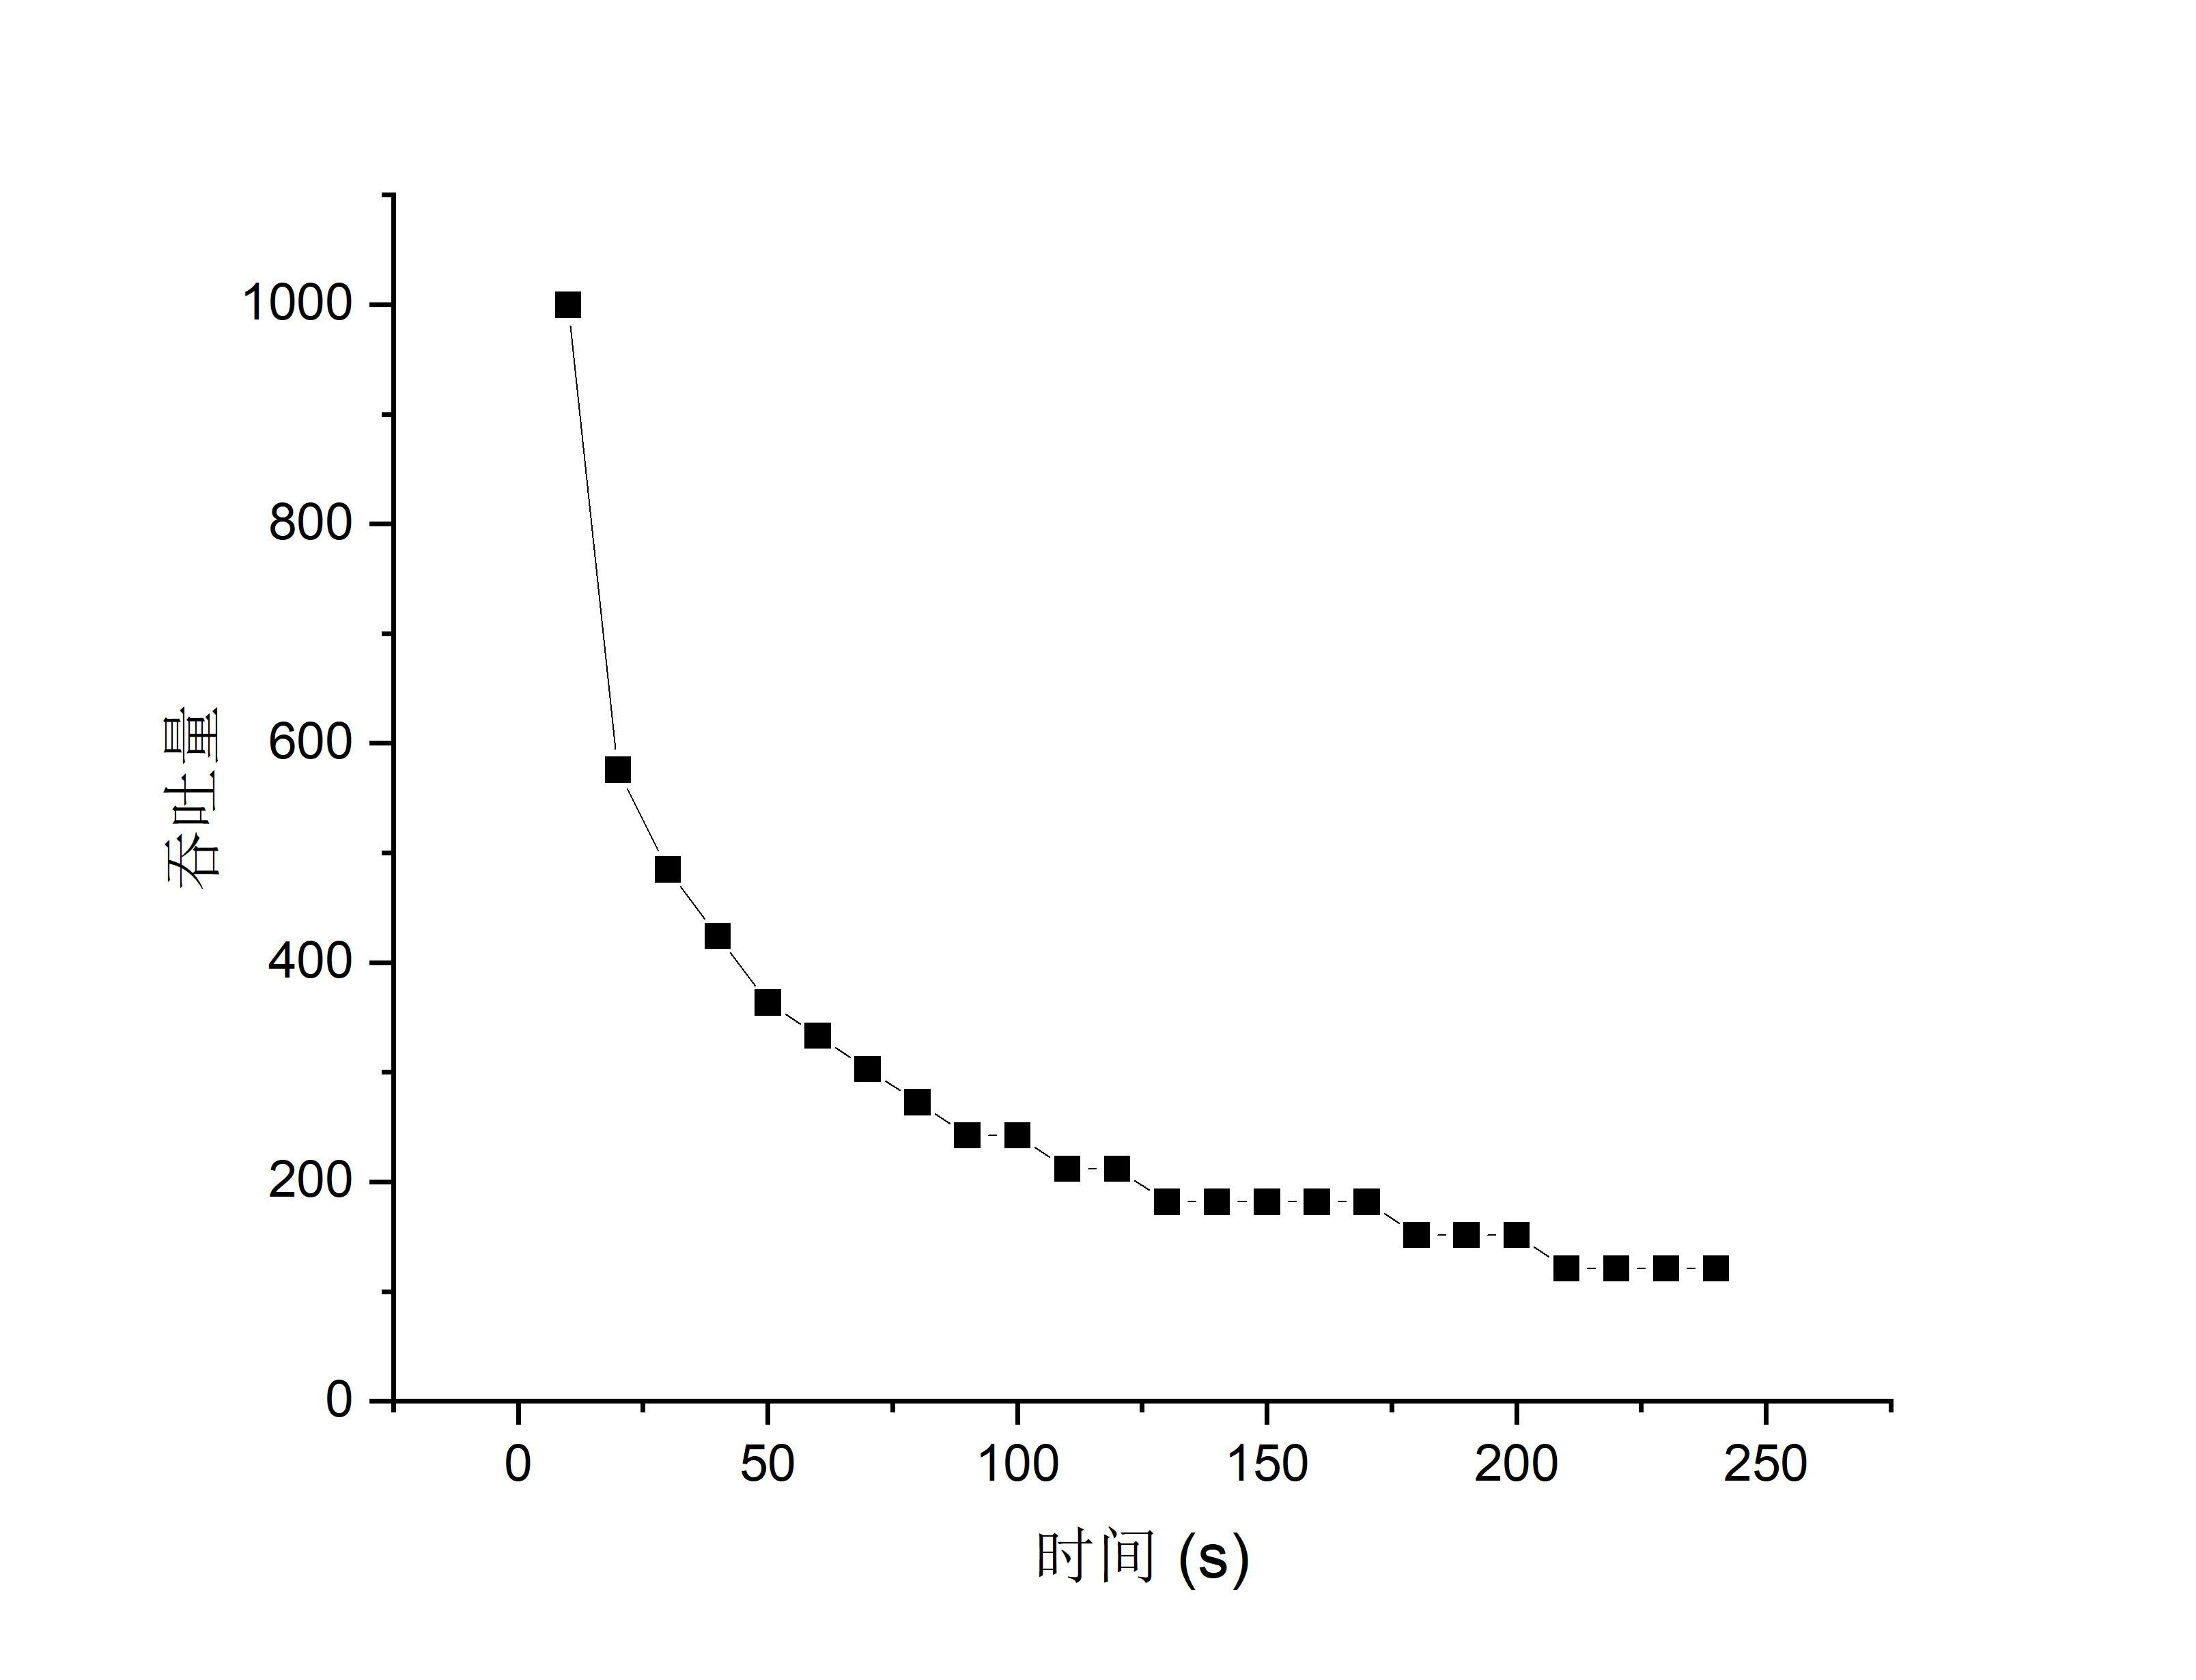
\includegraphics[scale=0.4]{graph1}
	\caption{持续插入过程中,PUT操作吞吐量随时间变化}
	\label{fig:1}
\end{figure}

整个插入过程共花费约260秒的时间。从图中我们可以明显看到,吞吐量随着时间呈现反比例下降趋势。这是符合预期的,因为在插入过程中,外存中的层级数越来越多,而每次合并操作都要合并到最后一层,导致平均吞吐量下降。

\subsubsection{对比实验}
%在此前的测试中,我们使用跳表实现了 MemTable。另外一种方法是使用 std::map 实现 MemTable。请通过实验数据,比较这两种实现对键值存储系统的性能影响,并给出建议(哪个更好或者什么时候该用哪个)。对比中应至少考虑到 PUT、GET、DEL 三个操作的性能。

上面的几节,我们专注于外存的性能,而对于内存而言,我们再本项目中采用的跳表,可能并不是最优的选择,还可以选择std::map等键值存储数据结构。在本节中,我们就对两者进行性能上的比较。实验数据采取与\ref{test}中的实验一相同的方案。

测试结果如表\ref{tab:4}所示(单位:秒)。

\begin{table}[ht]
	\caption{两种数据结构作为MemTable的性能对比}
	\label{tab:4}
	\begin{minipage}{0.5\textwidth}
		\begin{center}
			\begin{tabular}{c | c | c | c}
				\hline
				n & PUT & GET & DEL \\
				\hline\hline
				5,120 & 0.398 & 0.366 & 0.422 \\
				10,240 & 1.566 & 1.029 & 1.038 \\
				20,480 & 9.962 & 3.552 & 4.951 \\
				\hline
			\end{tabular}
			\captionof*{table}{跳表}
		\end{center}
	\end{minipage}
	\begin{minipage}{0.5\textwidth}
		\begin{center}
			\begin{tabular}{c | c | c | c}
				\hline
				n & PUT & GET & DEL \\
				\hline\hline
				5,120 & 0.480 & 0.331 & 0.336 \\
				10,240 & 1.615 & 0.899 & 0.926 \\
				20,480 & 9.839 & 3.982 & 4.126 \\
				\hline
			\end{tabular}
			\captionof*{table}{std::map}
		\end{center}
	\end{minipage}
\end{table}

从两表的对比中,我们看到其实两者的性能差异并不大,因为在平均意义上来说,两种数据结构的时间复杂度是一样的。由此合理推测,由于主要的时间花费在外存操作上,故所有具有对数级别的查询,插入,删除性能的数据结构,理论上应该都会得到类似的性能表现。

\section{结论}
LSM-KV键值存储系统是一种快速高效的键值管理系统。在本实验报告中,我们对该数据结构的内存、外存两部分分别进行了不同方面的测试。我们得出以下几个结论。

\begin{enumerate}
	\item 随着系统中已存储数据量的增大,LSM的性能逐渐降低,单次操作需要的平均时间更长,单种操作的平均吞吐量也会下降。
	\item 在内存中对所有SSTable中的索引信息和Bloom Filter 信息进行缓存是有必要的,能够显著提高相同条件下,LSM的平均吞吐量和综合性能。
	\item 内存数据结构采用std::map或跳表实现,效率差异不大。
\end{enumerate}

\section{致谢}

%在此部分中,你需要列出项目过程中所受到的帮助并进行致谢,包括但不限于从同学、朋友、开源项目、论坛、博客等处获得的启发和帮助。注意,此处不包括老师和助教。

经过一两个月的努力,我终于把LSM-KV数据结构实现了,并且进行了初步的优化。在此过程中,有许多同学给了我很多帮助,包括杨景凯,冯逸飞,董琛等等。在此,我表示对以上同学的感谢。



\section{其他和建议}
我觉得这个项目最大的坑就在于,我开始使用了好多vector,但是后来发现list和vector在默写情况下就是不能互相替代,比如如果有在中间插入的需求,那么vector虽然也可以实现,但是不是一个合理的选择,所以必须要谨慎选择数据结构。

另外,我起初不敢使用vector$\langle$pair$\langle$uint64\_t, list$\langle$pair$\langle$uint64\_t, string$\rangle$$\rangle$$\rangle$$\rangle$ 这种超长的复杂数据结构,后来被证明是必要的。。


\end{document}
